\documentclass[twoside]{book}

% Packages required by doxygen
\usepackage{fixltx2e}
\usepackage{calc}
\usepackage{doxygen}
\usepackage[export]{adjustbox} % also loads graphicx
\usepackage{graphicx}
\usepackage[utf8]{inputenc}
\usepackage{makeidx}
\usepackage{multicol}
\usepackage{multirow}
\PassOptionsToPackage{warn}{textcomp}
\usepackage{textcomp}
\usepackage[nointegrals]{wasysym}
\usepackage[table]{xcolor}

% Font selection
\usepackage[T1]{fontenc}
\usepackage[scaled=.90]{helvet}
\usepackage{courier}
\usepackage{amssymb}
\usepackage{sectsty}
\renewcommand{\familydefault}{\sfdefault}
\allsectionsfont{%
  \fontseries{bc}\selectfont%
  \color{darkgray}%
}
\renewcommand{\DoxyLabelFont}{%
  \fontseries{bc}\selectfont%
  \color{darkgray}%
}
\newcommand{\+}{\discretionary{\mbox{\scriptsize$\hookleftarrow$}}{}{}}

% Page & text layout
\usepackage{geometry}
\geometry{%
  a4paper,%
  top=2.5cm,%
  bottom=2.5cm,%
  left=2.5cm,%
  right=2.5cm%
}
\tolerance=750
\hfuzz=15pt
\hbadness=750
\setlength{\emergencystretch}{15pt}
\setlength{\parindent}{0cm}
\setlength{\parskip}{3ex plus 2ex minus 2ex}
\makeatletter
\renewcommand{\paragraph}{%
  \@startsection{paragraph}{4}{0ex}{-1.0ex}{1.0ex}{%
    \normalfont\normalsize\bfseries\SS@parafont%
  }%
}
\renewcommand{\subparagraph}{%
  \@startsection{subparagraph}{5}{0ex}{-1.0ex}{1.0ex}{%
    \normalfont\normalsize\bfseries\SS@subparafont%
  }%
}
\makeatother

% Headers & footers
\usepackage{fancyhdr}
\pagestyle{fancyplain}
\fancyhead[LE]{\fancyplain{}{\bfseries\thepage}}
\fancyhead[CE]{\fancyplain{}{}}
\fancyhead[RE]{\fancyplain{}{\bfseries\leftmark}}
\fancyhead[LO]{\fancyplain{}{\bfseries\rightmark}}
\fancyhead[CO]{\fancyplain{}{}}
\fancyhead[RO]{\fancyplain{}{\bfseries\thepage}}
\fancyfoot[LE]{\fancyplain{}{}}
\fancyfoot[CE]{\fancyplain{}{}}
\fancyfoot[RE]{\fancyplain{}{\bfseries\scriptsize Generated by Doxygen }}
\fancyfoot[LO]{\fancyplain{}{\bfseries\scriptsize Generated by Doxygen }}
\fancyfoot[CO]{\fancyplain{}{}}
\fancyfoot[RO]{\fancyplain{}{}}
\renewcommand{\footrulewidth}{0.4pt}
\renewcommand{\chaptermark}[1]{%
  \markboth{#1}{}%
}
\renewcommand{\sectionmark}[1]{%
  \markright{\thesection\ #1}%
}

% Indices & bibliography
\usepackage{natbib}
\usepackage[titles]{tocloft}
\setcounter{tocdepth}{3}
\setcounter{secnumdepth}{5}
\makeindex

% Hyperlinks (required, but should be loaded last)
\usepackage{ifpdf}
\ifpdf
  \usepackage[pdftex,pagebackref=true]{hyperref}
\else
  \usepackage[ps2pdf,pagebackref=true]{hyperref}
\fi
\hypersetup{%
  colorlinks=true,%
  linkcolor=blue,%
  citecolor=blue,%
  unicode%
}

% Custom commands
\newcommand{\clearemptydoublepage}{%
  \newpage{\pagestyle{empty}\cleardoublepage}%
}

\usepackage{caption}
\captionsetup{labelsep=space,justification=centering,font={bf},singlelinecheck=off,skip=4pt,position=top}

%===== C O N T E N T S =====

\begin{document}

% Titlepage & ToC
\hypersetup{pageanchor=false,
             bookmarksnumbered=true,
             pdfencoding=unicode
            }
\pagenumbering{alph}
\begin{titlepage}
\vspace*{7cm}
\begin{center}%
{\Large Akamai Analyzer \\[1ex]\large 1.\+0 }\\
\vspace*{1cm}
{\large Generated by Doxygen 1.8.14}\\
\end{center}
\end{titlepage}
\clearemptydoublepage
\pagenumbering{roman}
\tableofcontents
\clearemptydoublepage
\pagenumbering{arabic}
\hypersetup{pageanchor=true}

%--- Begin generated contents ---
\chapter{Hierarchical Index}
\section{Class Hierarchy}
This inheritance list is sorted roughly, but not completely, alphabetically\+:\begin{DoxyCompactList}
\item \contentsline{section}{Analyzer}{\pageref{class_analyzer}}{}
\begin{DoxyCompactList}
\item \contentsline{section}{Chain\+Analyzer}{\pageref{class_chain_analyzer}}{}
\item \contentsline{section}{Geo\+Perf\+Analyzer}{\pageref{class_geo_perf_analyzer}}{}
\end{DoxyCompactList}
\item iterator\begin{DoxyCompactList}
\item \contentsline{section}{Time\+Series$<$ T $>$\+:\+:iterator}{\pageref{class_time_series_1_1iterator}}{}
\end{DoxyCompactList}
\item \contentsline{section}{Network\+Info}{\pageref{struct_network_info}}{}
\item \contentsline{section}{Time\+Curve}{\pageref{class_time_curve}}{}
\item \contentsline{section}{Time\+Series$<$ T $>$}{\pageref{class_time_series}}{}
\item \contentsline{section}{Time\+Series$<$ T $>$\+:\+:timeslot}{\pageref{struct_time_series_1_1timeslot}}{}
\item \contentsline{section}{Tx}{\pageref{struct_tx}}{}
\item \contentsline{section}{Tx\+Set\+Calculator}{\pageref{class_tx_set_calculator}}{}
\item \contentsline{section}{Typed\+Extractor$<$ T $>$}{\pageref{struct_typed_extractor}}{}
\item \contentsline{section}{Typed\+Extractor$<$ std\+:\+:string $>$}{\pageref{struct_typed_extractor_3_01std_1_1string_01_4}}{}
\end{DoxyCompactList}

\chapter{Class Index}
\section{Class List}
Here are the classes, structs, unions and interfaces with brief descriptions\+:\begin{DoxyCompactList}
\item\contentsline{section}{\mbox{\hyperlink{class_analyzer}{Analyzer}} }{\pageref{class_analyzer}}{}
\item\contentsline{section}{\mbox{\hyperlink{class_chain_analyzer}{Chain\+Analyzer}} }{\pageref{class_chain_analyzer}}{}
\item\contentsline{section}{\mbox{\hyperlink{class_geo_perf_analyzer}{Geo\+Perf\+Analyzer}} }{\pageref{class_geo_perf_analyzer}}{}
\item\contentsline{section}{\mbox{\hyperlink{class_time_series_1_1iterator}{Time\+Series$<$ T $>$\+::iterator}} }{\pageref{class_time_series_1_1iterator}}{}
\item\contentsline{section}{\mbox{\hyperlink{struct_network_info}{Network\+Info}} }{\pageref{struct_network_info}}{}
\item\contentsline{section}{\mbox{\hyperlink{class_time_curve}{Time\+Curve}} }{\pageref{class_time_curve}}{}
\item\contentsline{section}{\mbox{\hyperlink{class_time_series}{Time\+Series$<$ T $>$}} }{\pageref{class_time_series}}{}
\item\contentsline{section}{\mbox{\hyperlink{struct_time_series_1_1timeslot}{Time\+Series$<$ T $>$\+::timeslot}} }{\pageref{struct_time_series_1_1timeslot}}{}
\item\contentsline{section}{\mbox{\hyperlink{struct_tx}{Tx}} }{\pageref{struct_tx}}{}
\item\contentsline{section}{\mbox{\hyperlink{class_tx_set_calculator}{Tx\+Set\+Calculator}} }{\pageref{class_tx_set_calculator}}{}
\item\contentsline{section}{\mbox{\hyperlink{struct_typed_extractor}{Typed\+Extractor$<$ T $>$}} }{\pageref{struct_typed_extractor}}{}
\item\contentsline{section}{\mbox{\hyperlink{struct_typed_extractor_3_01std_1_1string_01_4}{Typed\+Extractor$<$ std\+::string $>$}} }{\pageref{struct_typed_extractor_3_01std_1_1string_01_4}}{}
\end{DoxyCompactList}

\chapter{File Index}
\section{File List}
Here is a list of all documented files with brief descriptions\+:\begin{DoxyCompactList}
\item\contentsline{section}{/\+Users/ccheng/\+Documents/projects/akamai\+\_\+analyzer/src/{\bfseries Analyzer.\+h} }{\pageref{_analyzer_8h}}{}
\item\contentsline{section}{/\+Users/ccheng/\+Documents/projects/akamai\+\_\+analyzer/src/\mbox{\hyperlink{analyzermain_8cpp}{analyzermain.\+cpp}} }{\pageref{analyzermain_8cpp}}{}
\item\contentsline{section}{/\+Users/ccheng/\+Documents/projects/akamai\+\_\+analyzer/src/{\bfseries Chain\+Analyzer.\+h} }{\pageref{_chain_analyzer_8h}}{}
\item\contentsline{section}{/\+Users/ccheng/\+Documents/projects/akamai\+\_\+analyzer/src/{\bfseries Geo\+Perf\+Analyzer.\+h} }{\pageref{_geo_perf_analyzer_8h}}{}
\item\contentsline{section}{/\+Users/ccheng/\+Documents/projects/akamai\+\_\+analyzer/src/{\bfseries Network\+Info.\+h} }{\pageref{_network_info_8h}}{}
\item\contentsline{section}{/\+Users/ccheng/\+Documents/projects/akamai\+\_\+analyzer/src/{\bfseries Time\+Curve.\+h} }{\pageref{_time_curve_8h}}{}
\item\contentsline{section}{/\+Users/ccheng/\+Documents/projects/akamai\+\_\+analyzer/src/{\bfseries Time\+Series.\+h} }{\pageref{_time_series_8h}}{}
\item\contentsline{section}{/\+Users/ccheng/\+Documents/projects/akamai\+\_\+analyzer/src/{\bfseries Tx.\+h} }{\pageref{_tx_8h}}{}
\item\contentsline{section}{/\+Users/ccheng/\+Documents/projects/akamai\+\_\+analyzer/src/{\bfseries Tx\+Set\+Calculator.\+h} }{\pageref{_tx_set_calculator_8h}}{}
\item\contentsline{section}{/\+Users/ccheng/\+Documents/projects/akamai\+\_\+analyzer/src/{\bfseries utilities.\+h} }{\pageref{utilities_8h}}{}
\end{DoxyCompactList}

\chapter{Class Documentation}
\hypertarget{class_analyzer}{}\section{Analyzer Class Reference}
\label{class_analyzer}\index{Analyzer@{Analyzer}}


{\ttfamily \#include $<$Analyzer.\+h$>$}

Inheritance diagram for Analyzer\+:\begin{figure}[H]
\begin{center}
\leavevmode
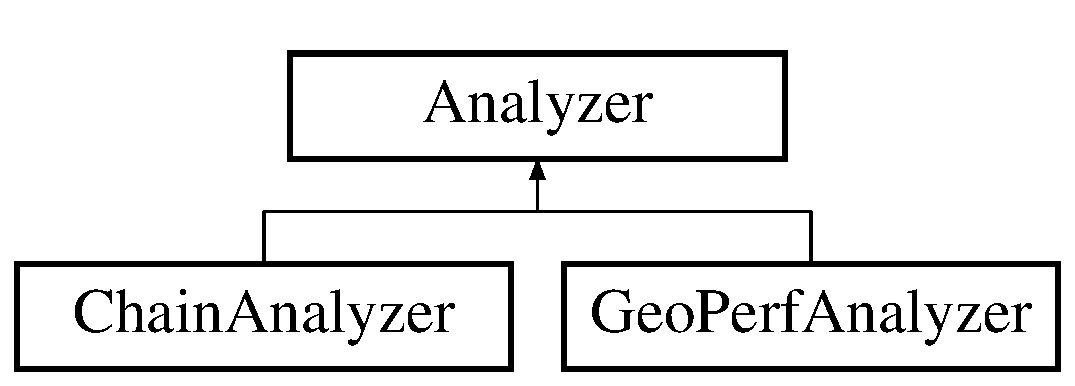
\includegraphics[height=2.000000cm]{class_analyzer}
\end{center}
\end{figure}
\subsection*{Public Types}
\begin{DoxyCompactItemize}
\item 
\mbox{\Hypertarget{class_analyzer_ab7e9cc7fdf79f6d9d40130dcb7a6c2e9}\label{class_analyzer_ab7e9cc7fdf79f6d9d40130dcb7a6c2e9}} 
enum {\bfseries Analyze\+Status} \{ {\bfseries A\+L\+L\+\_\+\+G\+O\+OD}, 
{\bfseries U\+N\+K\+N\+O\+W\+N\+\_\+\+L\+O\+G\+\_\+\+F\+O\+R\+M\+AT}
 \}
\end{DoxyCompactItemize}
\subsection*{Public Member Functions}
\begin{DoxyCompactItemize}
\item 
\mbox{\Hypertarget{class_analyzer_a391ddc6ff8813f2af0a44339964dd182}\label{class_analyzer_a391ddc6ff8813f2af0a44339964dd182}} 
void {\bfseries initialize} (int argc, char $\ast$$\ast$argv)
\item 
\mbox{\Hypertarget{class_analyzer_a236a6be53e03337ebc03a53883b0c0c9}\label{class_analyzer_a236a6be53e03337ebc03a53883b0c0c9}} 
void {\bfseries initialize} (\mbox{\hyperlink{struct_network_info}{Network\+Info}} n)
\item 
\mbox{\Hypertarget{class_analyzer_aea72fb1427846f406803266bb63484bf}\label{class_analyzer_aea72fb1427846f406803266bb63484bf}} 
virtual int {\bfseries parse} (vector$<$ string $>$)=0
\item 
\mbox{\Hypertarget{class_analyzer_a04ddbf427fc7fdc45b367cb04353b67a}\label{class_analyzer_a04ddbf427fc7fdc45b367cb04353b67a}} 
virtual void {\bfseries analyze} ()=0
\item 
\mbox{\Hypertarget{class_analyzer_a5ac5b45598e4e05ccce9df87fc6ddfd8}\label{class_analyzer_a5ac5b45598e4e05ccce9df87fc6ddfd8}} 
virtual void {\bfseries publish} ()=0
\item 
\mbox{\Hypertarget{class_analyzer_a0fc82817f3b75c6a0968135675c1b3d1}\label{class_analyzer_a0fc82817f3b75c6a0968135675c1b3d1}} 
virtual string {\bfseries get\+Error} ()=0
\item 
\mbox{\Hypertarget{class_analyzer_a19cd65a7c0abd2fdb8b285d9a0561321}\label{class_analyzer_a19cd65a7c0abd2fdb8b285d9a0561321}} 
string {\bfseries get\+Name} ()
\end{DoxyCompactItemize}


\subsection{Detailed Description}
Virtual base class for all analyzers 

The documentation for this class was generated from the following file\+:\begin{DoxyCompactItemize}
\item 
/\+Users/ccheng/\+Documents/projects/akamai\+\_\+analyzer/src/Analyzer.\+h\end{DoxyCompactItemize}

\hypertarget{class_chain_analyzer}{}\section{Chain\+Analyzer Class Reference}
\label{class_chain_analyzer}\index{Chain\+Analyzer@{Chain\+Analyzer}}


{\ttfamily \#include $<$Chain\+Analyzer.\+h$>$}

Inheritance diagram for Chain\+Analyzer\+:\begin{figure}[H]
\begin{center}
\leavevmode
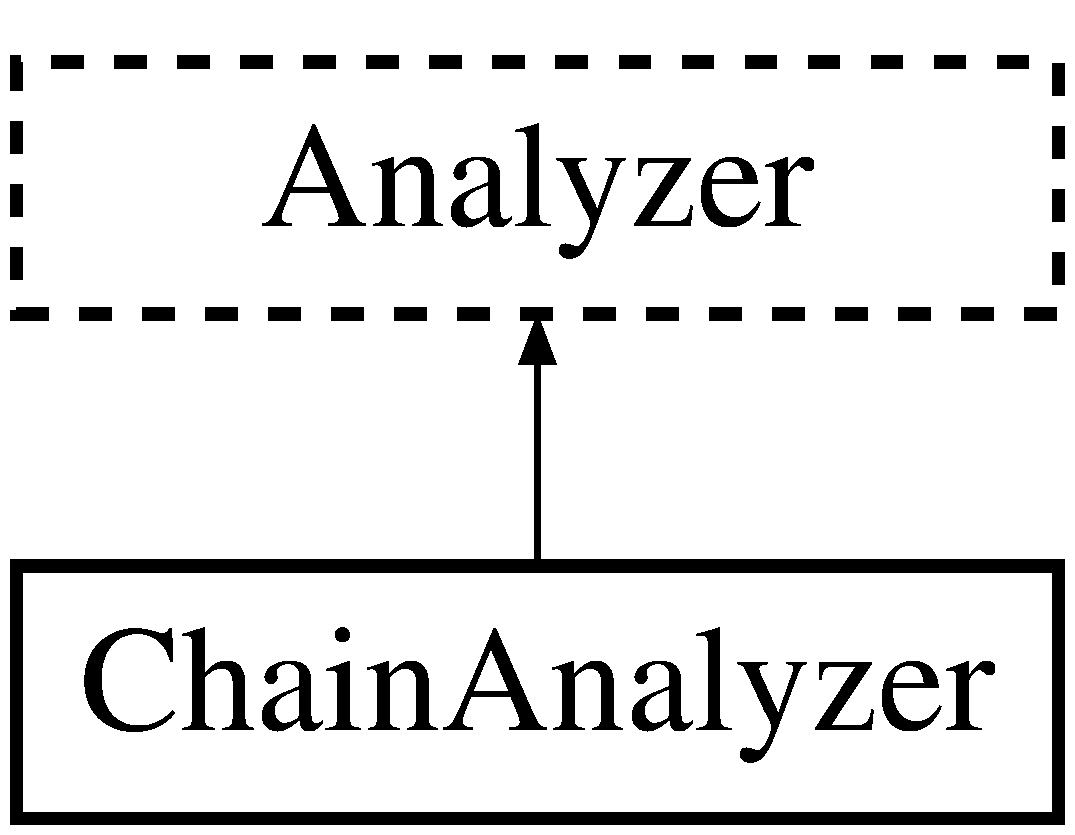
\includegraphics[height=2.000000cm]{class_chain_analyzer}
\end{center}
\end{figure}
\subsection*{Public Member Functions}
\begin{DoxyCompactItemize}
\item 
\mbox{\hyperlink{class_chain_analyzer_a5838d995d24865111ad93c07159eea70}{Chain\+Analyzer}} ()
\item 
\mbox{\hyperlink{class_chain_analyzer_a73079c72ffaf87957854ff6623830d6b}{$\sim$\+Chain\+Analyzer}} ()
\item 
void \mbox{\hyperlink{class_chain_analyzer_aac68bba73899bc53d6cd3c05877d9f85}{initialize}} (int, char $\ast$$\ast$)
\item 
void \mbox{\hyperlink{class_chain_analyzer_a1252905ce86f9e730263b083f85909f9}{initialize}} (\mbox{\hyperlink{struct_network_info}{Network\+Info}})
\item 
int \mbox{\hyperlink{class_chain_analyzer_a1beb2eb3b6bb4d12134e27b0328d8947}{parse\+String}} (string)
\item 
int \mbox{\hyperlink{class_chain_analyzer_a8ab1d495a31f6ec82544165d18f34d01}{parse}} (vector$<$ string $>$)
\item 
void \mbox{\hyperlink{class_chain_analyzer_a48f4f1f65d4eb2bd551ec6895b41ff51}{add\+Analyzer}} ()
\item 
void \mbox{\hyperlink{class_chain_analyzer_a836517181436aa5402ddd01374a496dd}{remove\+Analyzer}} ()
\item 
void \mbox{\hyperlink{class_chain_analyzer_a01d1323c8b1ef850d299c5625c2c97f2}{analyze}} ()
\item 
void \mbox{\hyperlink{class_chain_analyzer_a37568296a227c8f859917e765ab05dc2}{publish}} ()
\item 
string \mbox{\hyperlink{class_chain_analyzer_ae8cd5d49f3f41c4fd25baea14a80f929}{get\+Error}} ()
\end{DoxyCompactItemize}
\subsection*{Additional Inherited Members}


\subsection{Detailed Description}
A container analyzer working on the chain model 

\subsection{Constructor \& Destructor Documentation}
\mbox{\Hypertarget{class_chain_analyzer_a5838d995d24865111ad93c07159eea70}\label{class_chain_analyzer_a5838d995d24865111ad93c07159eea70}} 
\index{Chain\+Analyzer@{Chain\+Analyzer}!Chain\+Analyzer@{Chain\+Analyzer}}
\index{Chain\+Analyzer@{Chain\+Analyzer}!Chain\+Analyzer@{Chain\+Analyzer}}
\subsubsection{\texorpdfstring{Chain\+Analyzer()}{ChainAnalyzer()}}
{\footnotesize\ttfamily Chain\+Analyzer\+::\+Chain\+Analyzer (\begin{DoxyParamCaption}{ }\end{DoxyParamCaption})}

Constructor


\begin{DoxyParams}{Parameters}
{\em } & \\
\hline
\end{DoxyParams}
\mbox{\Hypertarget{class_chain_analyzer_a73079c72ffaf87957854ff6623830d6b}\label{class_chain_analyzer_a73079c72ffaf87957854ff6623830d6b}} 
\index{Chain\+Analyzer@{Chain\+Analyzer}!````~Chain\+Analyzer@{$\sim$\+Chain\+Analyzer}}
\index{````~Chain\+Analyzer@{$\sim$\+Chain\+Analyzer}!Chain\+Analyzer@{Chain\+Analyzer}}
\subsubsection{\texorpdfstring{$\sim$\+Chain\+Analyzer()}{~ChainAnalyzer()}}
{\footnotesize\ttfamily Chain\+Analyzer\+::$\sim$\+Chain\+Analyzer (\begin{DoxyParamCaption}{ }\end{DoxyParamCaption})\hspace{0.3cm}{\ttfamily [default]}}

Destructor


\begin{DoxyParams}{Parameters}
{\em } & \\
\hline
\end{DoxyParams}


\subsection{Member Function Documentation}
\mbox{\Hypertarget{class_chain_analyzer_a48f4f1f65d4eb2bd551ec6895b41ff51}\label{class_chain_analyzer_a48f4f1f65d4eb2bd551ec6895b41ff51}} 
\index{Chain\+Analyzer@{Chain\+Analyzer}!add\+Analyzer@{add\+Analyzer}}
\index{add\+Analyzer@{add\+Analyzer}!Chain\+Analyzer@{Chain\+Analyzer}}
\subsubsection{\texorpdfstring{add\+Analyzer()}{addAnalyzer()}}
{\footnotesize\ttfamily void Chain\+Analyzer\+::add\+Analyzer (\begin{DoxyParamCaption}{ }\end{DoxyParamCaption})}

Add analyzer into the chain


\begin{DoxyParams}{Parameters}
{\em } & \\
\hline
\end{DoxyParams}
\mbox{\Hypertarget{class_chain_analyzer_a01d1323c8b1ef850d299c5625c2c97f2}\label{class_chain_analyzer_a01d1323c8b1ef850d299c5625c2c97f2}} 
\index{Chain\+Analyzer@{Chain\+Analyzer}!analyze@{analyze}}
\index{analyze@{analyze}!Chain\+Analyzer@{Chain\+Analyzer}}
\subsubsection{\texorpdfstring{analyze()}{analyze()}}
{\footnotesize\ttfamily void Chain\+Analyzer\+::analyze (\begin{DoxyParamCaption}{ }\end{DoxyParamCaption})\hspace{0.3cm}{\ttfamily [virtual]}}

Analyze the parsed data to generate result


\begin{DoxyParams}{Parameters}
{\em } & \\
\hline
\end{DoxyParams}


Implements \mbox{\hyperlink{class_analyzer}{Analyzer}}.

\mbox{\Hypertarget{class_chain_analyzer_ae8cd5d49f3f41c4fd25baea14a80f929}\label{class_chain_analyzer_ae8cd5d49f3f41c4fd25baea14a80f929}} 
\index{Chain\+Analyzer@{Chain\+Analyzer}!get\+Error@{get\+Error}}
\index{get\+Error@{get\+Error}!Chain\+Analyzer@{Chain\+Analyzer}}
\subsubsection{\texorpdfstring{get\+Error()}{getError()}}
{\footnotesize\ttfamily string Chain\+Analyzer\+::get\+Error (\begin{DoxyParamCaption}{ }\end{DoxyParamCaption})\hspace{0.3cm}{\ttfamily [virtual]}}

Return the error message


\begin{DoxyParams}{Parameters}
{\em } & \\
\hline
\end{DoxyParams}


Implements \mbox{\hyperlink{class_analyzer}{Analyzer}}.

\mbox{\Hypertarget{class_chain_analyzer_aac68bba73899bc53d6cd3c05877d9f85}\label{class_chain_analyzer_aac68bba73899bc53d6cd3c05877d9f85}} 
\index{Chain\+Analyzer@{Chain\+Analyzer}!initialize@{initialize}}
\index{initialize@{initialize}!Chain\+Analyzer@{Chain\+Analyzer}}
\subsubsection{\texorpdfstring{initialize()}{initialize()}\hspace{0.1cm}{\footnotesize\ttfamily [1/2]}}
{\footnotesize\ttfamily void Chain\+Analyzer\+::initialize (\begin{DoxyParamCaption}\item[{int}]{argc,  }\item[{char $\ast$$\ast$}]{argv }\end{DoxyParamCaption})}

The initializer to setup the basic data structure according to the command line arguments


\begin{DoxyParams}{Parameters}
{\em } & \\
\hline
\end{DoxyParams}
\mbox{\Hypertarget{class_chain_analyzer_a1252905ce86f9e730263b083f85909f9}\label{class_chain_analyzer_a1252905ce86f9e730263b083f85909f9}} 
\index{Chain\+Analyzer@{Chain\+Analyzer}!initialize@{initialize}}
\index{initialize@{initialize}!Chain\+Analyzer@{Chain\+Analyzer}}
\subsubsection{\texorpdfstring{initialize()}{initialize()}\hspace{0.1cm}{\footnotesize\ttfamily [2/2]}}
{\footnotesize\ttfamily void Chain\+Analyzer\+::initialize (\begin{DoxyParamCaption}\item[{\mbox{\hyperlink{struct_network_info}{Network\+Info}}}]{n }\end{DoxyParamCaption})}

The initializer to setup the network info data structure


\begin{DoxyParams}{Parameters}
{\em } & \\
\hline
\end{DoxyParams}
\mbox{\Hypertarget{class_chain_analyzer_a8ab1d495a31f6ec82544165d18f34d01}\label{class_chain_analyzer_a8ab1d495a31f6ec82544165d18f34d01}} 
\index{Chain\+Analyzer@{Chain\+Analyzer}!parse@{parse}}
\index{parse@{parse}!Chain\+Analyzer@{Chain\+Analyzer}}
\subsubsection{\texorpdfstring{parse()}{parse()}}
{\footnotesize\ttfamily int Chain\+Analyzer\+::parse (\begin{DoxyParamCaption}\item[{vector$<$ string $>$}]{ts }\end{DoxyParamCaption})\hspace{0.3cm}{\ttfamily [virtual]}}

The data stream parser function to parse a (tokenized) string at a time


\begin{DoxyParams}{Parameters}
{\em } & \\
\hline
\end{DoxyParams}


Implements \mbox{\hyperlink{class_analyzer}{Analyzer}}.

\mbox{\Hypertarget{class_chain_analyzer_a1beb2eb3b6bb4d12134e27b0328d8947}\label{class_chain_analyzer_a1beb2eb3b6bb4d12134e27b0328d8947}} 
\index{Chain\+Analyzer@{Chain\+Analyzer}!parse\+String@{parse\+String}}
\index{parse\+String@{parse\+String}!Chain\+Analyzer@{Chain\+Analyzer}}
\subsubsection{\texorpdfstring{parse\+String()}{parseString()}}
{\footnotesize\ttfamily int Chain\+Analyzer\+::parse\+String (\begin{DoxyParamCaption}\item[{string}]{s }\end{DoxyParamCaption})}

The data stream parser function to parse a string at a time


\begin{DoxyParams}{Parameters}
{\em } & \\
\hline
\end{DoxyParams}
\mbox{\Hypertarget{class_chain_analyzer_a37568296a227c8f859917e765ab05dc2}\label{class_chain_analyzer_a37568296a227c8f859917e765ab05dc2}} 
\index{Chain\+Analyzer@{Chain\+Analyzer}!publish@{publish}}
\index{publish@{publish}!Chain\+Analyzer@{Chain\+Analyzer}}
\subsubsection{\texorpdfstring{publish()}{publish()}}
{\footnotesize\ttfamily void Chain\+Analyzer\+::publish (\begin{DoxyParamCaption}{ }\end{DoxyParamCaption})\hspace{0.3cm}{\ttfamily [virtual]}}

Publish result in a specified format to a specified output facility


\begin{DoxyParams}{Parameters}
{\em } & \\
\hline
\end{DoxyParams}


Implements \mbox{\hyperlink{class_analyzer}{Analyzer}}.

\mbox{\Hypertarget{class_chain_analyzer_a836517181436aa5402ddd01374a496dd}\label{class_chain_analyzer_a836517181436aa5402ddd01374a496dd}} 
\index{Chain\+Analyzer@{Chain\+Analyzer}!remove\+Analyzer@{remove\+Analyzer}}
\index{remove\+Analyzer@{remove\+Analyzer}!Chain\+Analyzer@{Chain\+Analyzer}}
\subsubsection{\texorpdfstring{remove\+Analyzer()}{removeAnalyzer()}}
{\footnotesize\ttfamily void Chain\+Analyzer\+::remove\+Analyzer (\begin{DoxyParamCaption}{ }\end{DoxyParamCaption})}

Remove analyzer from the chain


\begin{DoxyParams}{Parameters}
{\em } & \\
\hline
\end{DoxyParams}


The documentation for this class was generated from the following files\+:\begin{DoxyCompactItemize}
\item 
/\+Users/ccheng/\+Documents/projects/akamai\+\_\+analyzer/src/Chain\+Analyzer.\+h\item 
/\+Users/ccheng/\+Documents/projects/akamai\+\_\+analyzer/src/Chain\+Analyzer.\+cpp\end{DoxyCompactItemize}

\hypertarget{class_geo_perf_analyzer}{}\section{Geo\+Perf\+Analyzer Class Reference}
\label{class_geo_perf_analyzer}\index{Geo\+Perf\+Analyzer@{Geo\+Perf\+Analyzer}}


{\ttfamily \#include $<$Geo\+Perf\+Analyzer.\+h$>$}

Inheritance diagram for Geo\+Perf\+Analyzer\+:\begin{figure}[H]
\begin{center}
\leavevmode
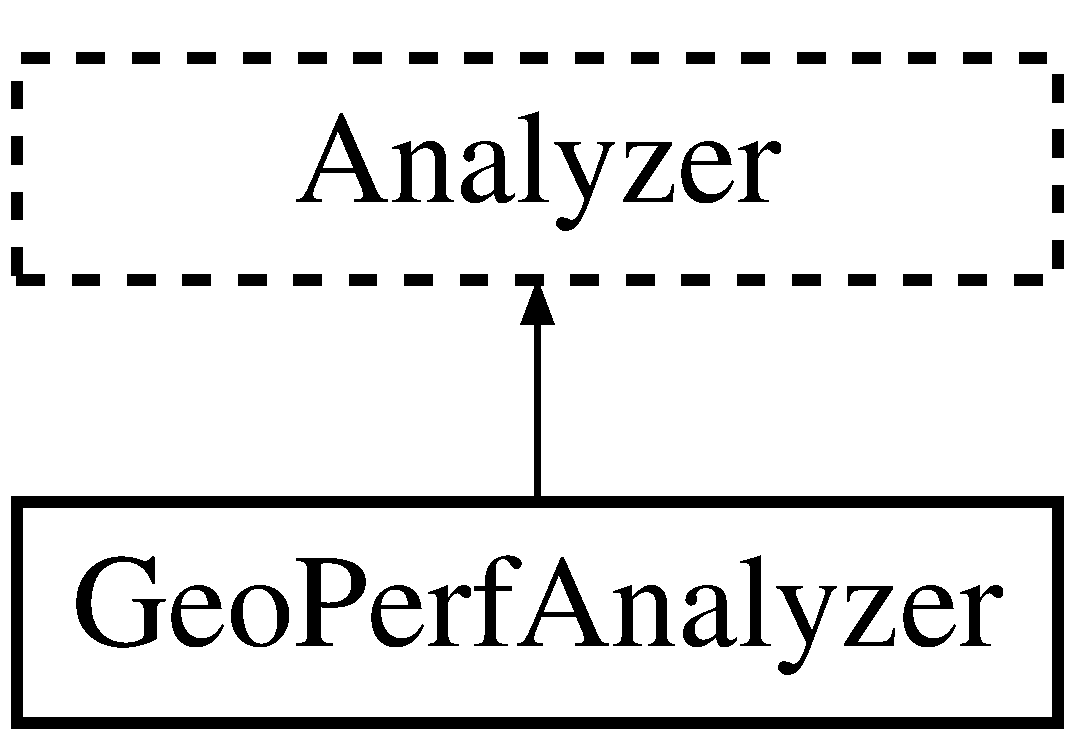
\includegraphics[height=2.000000cm]{class_geo_perf_analyzer}
\end{center}
\end{figure}
\subsection*{Public Member Functions}
\begin{DoxyCompactItemize}
\item 
\mbox{\hyperlink{class_geo_perf_analyzer_ac0414642cebe142c3d76c826978884c2}{Geo\+Perf\+Analyzer}} ()
\item 
\mbox{\hyperlink{class_geo_perf_analyzer_a91e810c076f5a79577698240af7c8dfd}{$\sim$\+Geo\+Perf\+Analyzer}} ()
\item 
void \mbox{\hyperlink{class_geo_perf_analyzer_aac29ab75a50ab1df9b9d49049ba96274}{initialize}} (int, char $\ast$$\ast$)
\item 
void \mbox{\hyperlink{class_geo_perf_analyzer_a4716557bfe06817b5d1c6c15e6a4e141}{initialize}} (\mbox{\hyperlink{struct_network_info}{Network\+Info}})
\item 
int \mbox{\hyperlink{class_geo_perf_analyzer_a03fcf5846ad4963692df9367e65469df}{parse}} (vector$<$ string $>$)
\item 
void \mbox{\hyperlink{class_geo_perf_analyzer_af62a34fd2e518e4505512318d2e56410}{analyze}} ()
\item 
void \mbox{\hyperlink{class_geo_perf_analyzer_af79f2adf101667172fd4b6c42459003c}{publish}} ()
\item 
string \mbox{\hyperlink{class_geo_perf_analyzer_a161e1261df25903eda37efe049975741}{get\+Error}} ()
\end{DoxyCompactItemize}
\subsection*{Protected Member Functions}
\begin{DoxyCompactItemize}
\item 
bool \mbox{\hyperlink{class_geo_perf_analyzer_a7259d409b07fc693bcc22a224c0e8c46}{isr\+Line}} (vector$<$ string $>$)
\item 
bool \mbox{\hyperlink{class_geo_perf_analyzer_a12fffe365c38eecb23093d3f7326cf79}{isf\+Line}} (vector$<$ string $>$)
\item 
\mbox{\Hypertarget{class_geo_perf_analyzer_a77bb6143e63e0ea5b87584714079bcb0}\label{class_geo_perf_analyzer_a77bb6143e63e0ea5b87584714079bcb0}} 
string {\bfseries compute\+Size\+String} (int)
\item 
\mbox{\Hypertarget{class_geo_perf_analyzer_a877ad78df3759dd3749f22e6352155f1}\label{class_geo_perf_analyzer_a877ad78df3759dd3749f22e6352155f1}} 
string {\bfseries make\+Key\+By\+Region} (string, string, int)
\item 
\mbox{\Hypertarget{class_geo_perf_analyzer_a451285e5235378bd904836a1baaeb22e}\label{class_geo_perf_analyzer_a451285e5235378bd904836a1baaeb22e}} 
string {\bfseries make\+Key\+By\+Geo} (string, string, int)
\end{DoxyCompactItemize}
\subsection*{Additional Inherited Members}


\subsection{Detailed Description}
A container analyzer working on the chain model 

\subsection{Constructor \& Destructor Documentation}
\mbox{\Hypertarget{class_geo_perf_analyzer_ac0414642cebe142c3d76c826978884c2}\label{class_geo_perf_analyzer_ac0414642cebe142c3d76c826978884c2}} 
\index{Geo\+Perf\+Analyzer@{Geo\+Perf\+Analyzer}!Geo\+Perf\+Analyzer@{Geo\+Perf\+Analyzer}}
\index{Geo\+Perf\+Analyzer@{Geo\+Perf\+Analyzer}!Geo\+Perf\+Analyzer@{Geo\+Perf\+Analyzer}}
\subsubsection{\texorpdfstring{Geo\+Perf\+Analyzer()}{GeoPerfAnalyzer()}}
{\footnotesize\ttfamily Geo\+Perf\+Analyzer\+::\+Geo\+Perf\+Analyzer (\begin{DoxyParamCaption}{ }\end{DoxyParamCaption})}

Constructor


\begin{DoxyParams}{Parameters}
{\em } & \\
\hline
\end{DoxyParams}
\mbox{\Hypertarget{class_geo_perf_analyzer_a91e810c076f5a79577698240af7c8dfd}\label{class_geo_perf_analyzer_a91e810c076f5a79577698240af7c8dfd}} 
\index{Geo\+Perf\+Analyzer@{Geo\+Perf\+Analyzer}!````~Geo\+Perf\+Analyzer@{$\sim$\+Geo\+Perf\+Analyzer}}
\index{````~Geo\+Perf\+Analyzer@{$\sim$\+Geo\+Perf\+Analyzer}!Geo\+Perf\+Analyzer@{Geo\+Perf\+Analyzer}}
\subsubsection{\texorpdfstring{$\sim$\+Geo\+Perf\+Analyzer()}{~GeoPerfAnalyzer()}}
{\footnotesize\ttfamily Geo\+Perf\+Analyzer\+::$\sim$\+Geo\+Perf\+Analyzer (\begin{DoxyParamCaption}{ }\end{DoxyParamCaption})\hspace{0.3cm}{\ttfamily [default]}}

Destructor


\begin{DoxyParams}{Parameters}
{\em } & \\
\hline
\end{DoxyParams}


\subsection{Member Function Documentation}
\mbox{\Hypertarget{class_geo_perf_analyzer_af62a34fd2e518e4505512318d2e56410}\label{class_geo_perf_analyzer_af62a34fd2e518e4505512318d2e56410}} 
\index{Geo\+Perf\+Analyzer@{Geo\+Perf\+Analyzer}!analyze@{analyze}}
\index{analyze@{analyze}!Geo\+Perf\+Analyzer@{Geo\+Perf\+Analyzer}}
\subsubsection{\texorpdfstring{analyze()}{analyze()}}
{\footnotesize\ttfamily void Geo\+Perf\+Analyzer\+::analyze (\begin{DoxyParamCaption}{ }\end{DoxyParamCaption})\hspace{0.3cm}{\ttfamily [virtual]}}

Analyze the parsed data to generate result


\begin{DoxyParams}{Parameters}
{\em } & \\
\hline
\end{DoxyParams}


Implements \mbox{\hyperlink{class_analyzer}{Analyzer}}.

\mbox{\Hypertarget{class_geo_perf_analyzer_a161e1261df25903eda37efe049975741}\label{class_geo_perf_analyzer_a161e1261df25903eda37efe049975741}} 
\index{Geo\+Perf\+Analyzer@{Geo\+Perf\+Analyzer}!get\+Error@{get\+Error}}
\index{get\+Error@{get\+Error}!Geo\+Perf\+Analyzer@{Geo\+Perf\+Analyzer}}
\subsubsection{\texorpdfstring{get\+Error()}{getError()}}
{\footnotesize\ttfamily string Geo\+Perf\+Analyzer\+::get\+Error (\begin{DoxyParamCaption}{ }\end{DoxyParamCaption})\hspace{0.3cm}{\ttfamily [virtual]}}

Return the error message


\begin{DoxyParams}{Parameters}
{\em } & \\
\hline
\end{DoxyParams}


Implements \mbox{\hyperlink{class_analyzer}{Analyzer}}.

\mbox{\Hypertarget{class_geo_perf_analyzer_aac29ab75a50ab1df9b9d49049ba96274}\label{class_geo_perf_analyzer_aac29ab75a50ab1df9b9d49049ba96274}} 
\index{Geo\+Perf\+Analyzer@{Geo\+Perf\+Analyzer}!initialize@{initialize}}
\index{initialize@{initialize}!Geo\+Perf\+Analyzer@{Geo\+Perf\+Analyzer}}
\subsubsection{\texorpdfstring{initialize()}{initialize()}\hspace{0.1cm}{\footnotesize\ttfamily [1/2]}}
{\footnotesize\ttfamily void Geo\+Perf\+Analyzer\+::initialize (\begin{DoxyParamCaption}\item[{int}]{argc,  }\item[{char $\ast$$\ast$}]{argv }\end{DoxyParamCaption})}

The initializer to setup the basic data structure according to the command line arguments


\begin{DoxyParams}{Parameters}
{\em } & \\
\hline
\end{DoxyParams}
\mbox{\Hypertarget{class_geo_perf_analyzer_a4716557bfe06817b5d1c6c15e6a4e141}\label{class_geo_perf_analyzer_a4716557bfe06817b5d1c6c15e6a4e141}} 
\index{Geo\+Perf\+Analyzer@{Geo\+Perf\+Analyzer}!initialize@{initialize}}
\index{initialize@{initialize}!Geo\+Perf\+Analyzer@{Geo\+Perf\+Analyzer}}
\subsubsection{\texorpdfstring{initialize()}{initialize()}\hspace{0.1cm}{\footnotesize\ttfamily [2/2]}}
{\footnotesize\ttfamily void Geo\+Perf\+Analyzer\+::initialize (\begin{DoxyParamCaption}\item[{\mbox{\hyperlink{struct_network_info}{Network\+Info}}}]{n }\end{DoxyParamCaption})}

The initializer to setup the network info data structure


\begin{DoxyParams}{Parameters}
{\em } & \\
\hline
\end{DoxyParams}
\mbox{\Hypertarget{class_geo_perf_analyzer_a12fffe365c38eecb23093d3f7326cf79}\label{class_geo_perf_analyzer_a12fffe365c38eecb23093d3f7326cf79}} 
\index{Geo\+Perf\+Analyzer@{Geo\+Perf\+Analyzer}!isf\+Line@{isf\+Line}}
\index{isf\+Line@{isf\+Line}!Geo\+Perf\+Analyzer@{Geo\+Perf\+Analyzer}}
\subsubsection{\texorpdfstring{isf\+Line()}{isfLine()}}
{\footnotesize\ttfamily bool Geo\+Perf\+Analyzer\+::isf\+Line (\begin{DoxyParamCaption}\item[{vector$<$ string $>$}]{ts }\end{DoxyParamCaption})\hspace{0.3cm}{\ttfamily [protected]}}

if it is an f line


\begin{DoxyParams}{Parameters}
{\em } & \\
\hline
\end{DoxyParams}
\mbox{\Hypertarget{class_geo_perf_analyzer_a7259d409b07fc693bcc22a224c0e8c46}\label{class_geo_perf_analyzer_a7259d409b07fc693bcc22a224c0e8c46}} 
\index{Geo\+Perf\+Analyzer@{Geo\+Perf\+Analyzer}!isr\+Line@{isr\+Line}}
\index{isr\+Line@{isr\+Line}!Geo\+Perf\+Analyzer@{Geo\+Perf\+Analyzer}}
\subsubsection{\texorpdfstring{isr\+Line()}{isrLine()}}
{\footnotesize\ttfamily bool Geo\+Perf\+Analyzer\+::isr\+Line (\begin{DoxyParamCaption}\item[{vector$<$ string $>$}]{ts }\end{DoxyParamCaption})\hspace{0.3cm}{\ttfamily [protected]}}

if it is an r line


\begin{DoxyParams}{Parameters}
{\em } & \\
\hline
\end{DoxyParams}
\mbox{\Hypertarget{class_geo_perf_analyzer_a03fcf5846ad4963692df9367e65469df}\label{class_geo_perf_analyzer_a03fcf5846ad4963692df9367e65469df}} 
\index{Geo\+Perf\+Analyzer@{Geo\+Perf\+Analyzer}!parse@{parse}}
\index{parse@{parse}!Geo\+Perf\+Analyzer@{Geo\+Perf\+Analyzer}}
\subsubsection{\texorpdfstring{parse()}{parse()}}
{\footnotesize\ttfamily int Geo\+Perf\+Analyzer\+::parse (\begin{DoxyParamCaption}\item[{vector$<$ string $>$}]{ts }\end{DoxyParamCaption})\hspace{0.3cm}{\ttfamily [virtual]}}

The data stream parser function to parse a (tokenized) string at a time


\begin{DoxyParams}{Parameters}
{\em } & \\
\hline
\end{DoxyParams}


Implements \mbox{\hyperlink{class_analyzer}{Analyzer}}.

\mbox{\Hypertarget{class_geo_perf_analyzer_af79f2adf101667172fd4b6c42459003c}\label{class_geo_perf_analyzer_af79f2adf101667172fd4b6c42459003c}} 
\index{Geo\+Perf\+Analyzer@{Geo\+Perf\+Analyzer}!publish@{publish}}
\index{publish@{publish}!Geo\+Perf\+Analyzer@{Geo\+Perf\+Analyzer}}
\subsubsection{\texorpdfstring{publish()}{publish()}}
{\footnotesize\ttfamily void Geo\+Perf\+Analyzer\+::publish (\begin{DoxyParamCaption}{ }\end{DoxyParamCaption})\hspace{0.3cm}{\ttfamily [virtual]}}

Publish result in a specified format to a specified output facility


\begin{DoxyParams}{Parameters}
{\em } & \\
\hline
\end{DoxyParams}


Implements \mbox{\hyperlink{class_analyzer}{Analyzer}}.



The documentation for this class was generated from the following files\+:\begin{DoxyCompactItemize}
\item 
/\+Users/ccheng/\+Documents/projects/akamai\+\_\+analyzer/src/Geo\+Perf\+Analyzer.\+h\item 
/\+Users/ccheng/\+Documents/projects/akamai\+\_\+analyzer/src/Geo\+Perf\+Analyzer.\+cpp\end{DoxyCompactItemize}

\hypertarget{class_time_series_1_1iterator}{}\section{Time\+Series$<$ T $>$\+:\+:iterator Class Reference}
\label{class_time_series_1_1iterator}\index{Time\+Series$<$ T $>$\+::iterator@{Time\+Series$<$ T $>$\+::iterator}}
Inheritance diagram for Time\+Series$<$ T $>$\+:\+:iterator\+:\begin{figure}[H]
\begin{center}
\leavevmode
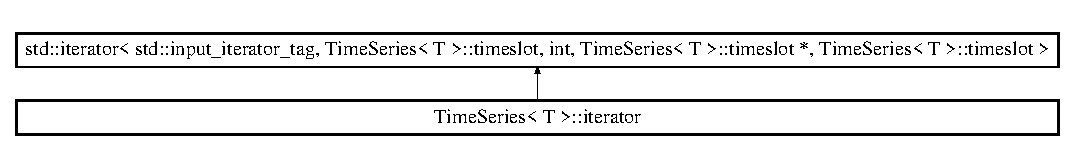
\includegraphics[height=1.584159cm]{class_time_series_1_1iterator}
\end{center}
\end{figure}
\subsection*{Public Member Functions}
\begin{DoxyCompactItemize}
\item 
\mbox{\Hypertarget{class_time_series_1_1iterator_a67884c3163708f5898d86c08d66f4e47}\label{class_time_series_1_1iterator_a67884c3163708f5898d86c08d66f4e47}} 
{\bfseries iterator} (\mbox{\hyperlink{class_time_series}{Time\+Series}}$<$ T $>$ $\ast$p, double \+\_\+timepoint=0)
\item 
\mbox{\Hypertarget{class_time_series_1_1iterator_a823ab3a7ba9e70776a3865a3b9f39113}\label{class_time_series_1_1iterator_a823ab3a7ba9e70776a3865a3b9f39113}} 
\mbox{\hyperlink{class_time_series_1_1iterator}{iterator}} \& {\bfseries operator++} ()
\item 
\mbox{\Hypertarget{class_time_series_1_1iterator_a1c47c88818865e05d37b7b5a42fc6c65}\label{class_time_series_1_1iterator_a1c47c88818865e05d37b7b5a42fc6c65}} 
\mbox{\hyperlink{class_time_series_1_1iterator}{iterator}} {\bfseries operator++} (int)
\item 
\mbox{\Hypertarget{class_time_series_1_1iterator_a9691ae899619277a4c3aa88b64166efc}\label{class_time_series_1_1iterator_a9691ae899619277a4c3aa88b64166efc}} 
bool {\bfseries operator==} (\mbox{\hyperlink{class_time_series_1_1iterator}{iterator}} other) const
\item 
\mbox{\Hypertarget{class_time_series_1_1iterator_a72462d4321fdb80297b8bd91b3896063}\label{class_time_series_1_1iterator_a72462d4321fdb80297b8bd91b3896063}} 
bool {\bfseries operator!=} (\mbox{\hyperlink{class_time_series_1_1iterator}{iterator}} other) const
\item 
\mbox{\Hypertarget{class_time_series_1_1iterator_a290d256ff98882a20f1ae34b63e8e29d}\label{class_time_series_1_1iterator_a290d256ff98882a20f1ae34b63e8e29d}} 
iterator\+\_\+traits$<$ \mbox{\hyperlink{class_time_series_1_1iterator}{iterator}} $>$\+::reference {\bfseries operator$\ast$} () const
\end{DoxyCompactItemize}


The documentation for this class was generated from the following file\+:\begin{DoxyCompactItemize}
\item 
/\+Users/ccheng/\+Documents/projects/akamai\+\_\+analyzer/src/Time\+Series.\+h\end{DoxyCompactItemize}

\hypertarget{struct_network_info}{}\section{Network\+Info Struct Reference}
\label{struct_network_info}\index{Network\+Info@{Network\+Info}}
\subsection*{Public Member Functions}
\begin{DoxyCompactItemize}
\item 
\mbox{\Hypertarget{struct_network_info_a44900ff326a66b38e655927ff3135e7d}\label{struct_network_info_a44900ff326a66b38e655927ff3135e7d}} 
bool {\bfseries is\+Empty} ()
\item 
\mbox{\Hypertarget{struct_network_info_a838d52f7f019e50c926752d2337b1d67}\label{struct_network_info_a838d52f7f019e50c926752d2337b1d67}} 
void {\bfseries init\+Ip\+To\+Region} (string csv\+\_\+file)
\item 
\mbox{\Hypertarget{struct_network_info_a3a2a6df513fcdf5e7dccb12582821175}\label{struct_network_info_a3a2a6df513fcdf5e7dccb12582821175}} 
void {\bfseries init\+Region\+To\+Geo} (string csv\+\_\+file)
\item 
\mbox{\Hypertarget{struct_network_info_aebae6f4c762ce6467a07fa6f702cc11c}\label{struct_network_info_aebae6f4c762ce6467a07fa6f702cc11c}} 
string {\bfseries get\+Region} (string IP)
\item 
\mbox{\Hypertarget{struct_network_info_aa034823ffc797fe3db64b46a9592747f}\label{struct_network_info_aa034823ffc797fe3db64b46a9592747f}} 
string {\bfseries get\+Geo} (string region)
\end{DoxyCompactItemize}
\subsection*{Public Attributes}
\begin{DoxyCompactItemize}
\item 
\mbox{\Hypertarget{struct_network_info_a234f8dac6c935838cdaa52e6b803cd1f}\label{struct_network_info_a234f8dac6c935838cdaa52e6b803cd1f}} 
map$<$ string, string $>$ {\bfseries Ip\+To\+Region}
\item 
\mbox{\Hypertarget{struct_network_info_ae85b2fca3d6ef8c021f5ba5d5a3e8cc9}\label{struct_network_info_ae85b2fca3d6ef8c021f5ba5d5a3e8cc9}} 
map$<$ string, string $>$ {\bfseries Region\+To\+Geo}
\end{DoxyCompactItemize}


The documentation for this struct was generated from the following file\+:\begin{DoxyCompactItemize}
\item 
/\+Users/ccheng/\+Documents/projects/akamai\+\_\+analyzer/src/Network\+Info.\+h\end{DoxyCompactItemize}

\hypertarget{class_time_curve}{}\section{Time\+Curve Class Reference}
\label{class_time_curve}\index{Time\+Curve@{Time\+Curve}}
\subsection*{Public Member Functions}
\begin{DoxyCompactItemize}
\item 
\mbox{\Hypertarget{class_time_curve_ac14b01b5912e595a5eabf7e18037182c}\label{class_time_curve_ac14b01b5912e595a5eabf7e18037182c}} 
{\bfseries Time\+Curve} (\mbox{\hyperlink{class_time_series}{Time\+Series}}$<$ \mbox{\hyperlink{struct_tx}{Tx}} $>$\+::iterator, \mbox{\hyperlink{class_time_series}{Time\+Series}}$<$ \mbox{\hyperlink{struct_tx}{Tx}} $>$\+::iterator, \mbox{\hyperlink{class_tx_set_calculator}{Tx\+Set\+Calculator}})
\item 
\mbox{\Hypertarget{class_time_curve_ae89faf04ad2058d22ab6bbda368db6ae}\label{class_time_curve_ae89faf04ad2058d22ab6bbda368db6ae}} 
map$<$ double, float $>$ {\bfseries get\+Curve} () const
\item 
\mbox{\Hypertarget{class_time_curve_a66215ed449760eec02fc4e5935ead88d}\label{class_time_curve_a66215ed449760eec02fc4e5935ead88d}} 
int {\bfseries get\+Full\+Count} () const
\item 
\mbox{\Hypertarget{class_time_curve_a125d2f564e6aef2b6fea42dab2d631aa}\label{class_time_curve_a125d2f564e6aef2b6fea42dab2d631aa}} 
int {\bfseries get\+Count} () const
\item 
\mbox{\Hypertarget{class_time_curve_a604f3be1ca972bc24d6e2b094a6da4e9}\label{class_time_curve_a604f3be1ca972bc24d6e2b094a6da4e9}} 
float {\bfseries get\+Max} () const
\item 
\mbox{\Hypertarget{class_time_curve_a28a1ea7f6f36fe41e6a59f21f022bcb9}\label{class_time_curve_a28a1ea7f6f36fe41e6a59f21f022bcb9}} 
float {\bfseries get\+Min} () const
\item 
\mbox{\Hypertarget{class_time_curve_a928370cfcc4300cee821c5b130777a6c}\label{class_time_curve_a928370cfcc4300cee821c5b130777a6c}} 
float {\bfseries get\+Avg} () const
\item 
\mbox{\Hypertarget{class_time_curve_af7e1addb63dd5c03f7b0e05474eb5192}\label{class_time_curve_af7e1addb63dd5c03f7b0e05474eb5192}} 
double {\bfseries get\+Start\+Time} () const
\item 
\mbox{\Hypertarget{class_time_curve_a19d11b7c6a01378ef3dc0f9449d56711}\label{class_time_curve_a19d11b7c6a01378ef3dc0f9449d56711}} 
double {\bfseries get\+End\+Time} () const
\item 
\mbox{\Hypertarget{class_time_curve_a3efa560bca5bc8db08cd66901a5763cf}\label{class_time_curve_a3efa560bca5bc8db08cd66901a5763cf}} 
double {\bfseries get\+Granularity} () const
\item 
\mbox{\Hypertarget{class_time_curve_afc64b4ed364377de075eee475dc41150}\label{class_time_curve_afc64b4ed364377de075eee475dc41150}} 
string {\bfseries to\+String} () const
\end{DoxyCompactItemize}


The documentation for this class was generated from the following files\+:\begin{DoxyCompactItemize}
\item 
/\+Users/ccheng/\+Documents/projects/akamai\+\_\+analyzer/src/Time\+Curve.\+h\item 
/\+Users/ccheng/\+Documents/projects/akamai\+\_\+analyzer/src/Time\+Curve.\+cpp\end{DoxyCompactItemize}

\hypertarget{class_time_series}{}\section{Time\+Series$<$ T $>$ Class Template Reference}
\label{class_time_series}\index{Time\+Series$<$ T $>$@{Time\+Series$<$ T $>$}}
\subsection*{Classes}
\begin{DoxyCompactItemize}
\item 
class \mbox{\hyperlink{class_time_series_1_1iterator}{iterator}}
\item 
struct \mbox{\hyperlink{struct_time_series_1_1timeslot}{timeslot}}
\end{DoxyCompactItemize}
\subsection*{Public Member Functions}
\begin{DoxyCompactItemize}
\item 
\mbox{\Hypertarget{class_time_series_aa2555a043f2e3d6bae3a752001073068}\label{class_time_series_aa2555a043f2e3d6bae3a752001073068}} 
{\bfseries Time\+Series} (double granularity)
\item 
\mbox{\Hypertarget{class_time_series_ac5f4941233217d3355f4835ca9fd5b1e}\label{class_time_series_ac5f4941233217d3355f4835ca9fd5b1e}} 
int {\bfseries time\+To\+Slot} (double time)
\item 
\mbox{\Hypertarget{class_time_series_afa51501890d20c04172d09d7fcc794cf}\label{class_time_series_afa51501890d20c04172d09d7fcc794cf}} 
bool {\bfseries exists} (double time, T obj)
\item 
\mbox{\Hypertarget{class_time_series_a3c91d1dc6f9cd508a6de650709200aa4}\label{class_time_series_a3c91d1dc6f9cd508a6de650709200aa4}} 
void {\bfseries add} (double time, T obj)
\item 
\mbox{\Hypertarget{class_time_series_a12cce7cc67e03364b64051cf4aadec72}\label{class_time_series_a12cce7cc67e03364b64051cf4aadec72}} 
void {\bfseries reset\+Min\+Max\+Slots} ()
\item 
\mbox{\Hypertarget{class_time_series_a57d69f1af93c7376f6fb9fd6b9cf284c}\label{class_time_series_a57d69f1af93c7376f6fb9fd6b9cf284c}} 
void {\bfseries remove} (T obj, double begin\+\_\+time=0, double end\+\_\+time=0)
\item 
\mbox{\Hypertarget{class_time_series_a52a961a7794a2890365e1b7107d5889c}\label{class_time_series_a52a961a7794a2890365e1b7107d5889c}} 
\mbox{\hyperlink{class_time_series_1_1iterator}{iterator}} {\bfseries begin} (double timepoint)
\item 
\mbox{\Hypertarget{class_time_series_a44ec9bc127afa154573678d9e4b48605}\label{class_time_series_a44ec9bc127afa154573678d9e4b48605}} 
\mbox{\hyperlink{class_time_series_1_1iterator}{iterator}} {\bfseries end} (double timepoint)
\end{DoxyCompactItemize}


The documentation for this class was generated from the following file\+:\begin{DoxyCompactItemize}
\item 
/\+Users/ccheng/\+Documents/projects/akamai\+\_\+analyzer/src/Time\+Series.\+h\end{DoxyCompactItemize}

\hypertarget{struct_time_series_1_1timeslot}{}\section{Time\+Series$<$ T $>$\+:\+:timeslot Struct Reference}
\label{struct_time_series_1_1timeslot}\index{Time\+Series$<$ T $>$\+::timeslot@{Time\+Series$<$ T $>$\+::timeslot}}
\subsection*{Public Attributes}
\begin{DoxyCompactItemize}
\item 
\mbox{\Hypertarget{struct_time_series_1_1timeslot_ae8f4583682c3aaad6faeaf9f33d6a049}\label{struct_time_series_1_1timeslot_ae8f4583682c3aaad6faeaf9f33d6a049}} 
double {\bfseries begin\+\_\+time}
\item 
\mbox{\Hypertarget{struct_time_series_1_1timeslot_afd515f71689dd357c69711f9275f9788}\label{struct_time_series_1_1timeslot_afd515f71689dd357c69711f9275f9788}} 
double {\bfseries end\+\_\+time}
\item 
\mbox{\Hypertarget{struct_time_series_1_1timeslot_afa4468e18eb7664e7c705969f92ad41b}\label{struct_time_series_1_1timeslot_afa4468e18eb7664e7c705969f92ad41b}} 
multimap$<$ double, T $>$ $\ast$ {\bfseries datapoints}
\end{DoxyCompactItemize}


The documentation for this struct was generated from the following file\+:\begin{DoxyCompactItemize}
\item 
/\+Users/ccheng/\+Documents/projects/akamai\+\_\+analyzer/src/Time\+Series.\+h\end{DoxyCompactItemize}

\hypertarget{struct_tx}{}\section{Tx Struct Reference}
\label{struct_tx}\index{Tx@{Tx}}
\subsection*{Public Member Functions}
\begin{DoxyCompactItemize}
\item 
\mbox{\Hypertarget{struct_tx_a8297da293985cedd19580a6f899af436}\label{struct_tx_a8297da293985cedd19580a6f899af436}} 
{\bfseries Tx} (vector$<$ string $>$ vs)
\item 
\mbox{\Hypertarget{struct_tx_a362b2020ac783b2196e0946e447a8083}\label{struct_tx_a362b2020ac783b2196e0946e447a8083}} 
bool {\bfseries has\+Valid\+Throughput} ()
\end{DoxyCompactItemize}
\subsection*{Public Attributes}
\begin{DoxyCompactItemize}
\item 
\mbox{\Hypertarget{struct_tx_a1cbd03a7ec5a0cc651666d0795e0548e}\label{struct_tx_a1cbd03a7ec5a0cc651666d0795e0548e}} 
int {\bfseries content\+\_\+size}
\item 
\mbox{\Hypertarget{struct_tx_a0181e88dbe6a9f42567e3153413deba0}\label{struct_tx_a0181e88dbe6a9f42567e3153413deba0}} 
int {\bfseries total\+\_\+size}
\item 
\mbox{\Hypertarget{struct_tx_a931b7d10a8b7f8da31339a6a55b28be9}\label{struct_tx_a931b7d10a8b7f8da31339a6a55b28be9}} 
int {\bfseries transfer\+\_\+time}
\item 
\mbox{\Hypertarget{struct_tx_aa1405c060e20c2c1a3a485349db3d735}\label{struct_tx_aa1405c060e20c2c1a3a485349db3d735}} 
int {\bfseries ssl\+\_\+time}
\item 
\mbox{\Hypertarget{struct_tx_ad9d8c7ebf3aa6396d734376cc0d913a5}\label{struct_tx_ad9d8c7ebf3aa6396d734376cc0d913a5}} 
int {\bfseries req\+\_\+end\+\_\+time}
\item 
\mbox{\Hypertarget{struct_tx_afe8c130ad6ffa633708cec477a3dab47}\label{struct_tx_afe8c130ad6ffa633708cec477a3dab47}} 
int {\bfseries turnaround\+\_\+time}
\item 
\mbox{\Hypertarget{struct_tx_a290fe930cd644d9cfd52ff61191c5f4a}\label{struct_tx_a290fe930cd644d9cfd52ff61191c5f4a}} 
string {\bfseries status\+\_\+code}
\item 
\mbox{\Hypertarget{struct_tx_add727365a75bc29e49a9247d981fc735}\label{struct_tx_add727365a75bc29e49a9247d981fc735}} 
string {\bfseries error\+\_\+code}
\item 
\mbox{\Hypertarget{struct_tx_a5bc03d1d0fb33044bda1d8387feca8b8}\label{struct_tx_a5bc03d1d0fb33044bda1d8387feca8b8}} 
string {\bfseries flag}
\item 
\mbox{\Hypertarget{struct_tx_ac99bd5b80964100fc5614f9ff8491120}\label{struct_tx_ac99bd5b80964100fc5614f9ff8491120}} 
double {\bfseries timestamp}
\item 
\mbox{\Hypertarget{struct_tx_a2792502a06d590ee17cab0ad2c0f06e9}\label{struct_tx_a2792502a06d590ee17cab0ad2c0f06e9}} 
string {\bfseries req\+\_\+id}
\item 
\mbox{\Hypertarget{struct_tx_a147834eb940da2b7eaae1fd89114dfc5}\label{struct_tx_a147834eb940da2b7eaae1fd89114dfc5}} 
string {\bfseries arl}
\item 
\mbox{\Hypertarget{struct_tx_ab25e8628ee0d7b707193eff708f2bc31}\label{struct_tx_ab25e8628ee0d7b707193eff708f2bc31}} 
string {\bfseries byte\+\_\+range}
\item 
\mbox{\Hypertarget{struct_tx_a0417366565b08f605194bba01cff1a5c}\label{struct_tx_a0417366565b08f605194bba01cff1a5c}} 
string {\bfseries ghost\+\_\+ip}
\item 
\mbox{\Hypertarget{struct_tx_a2f5439a7da3cda247c552c29194f3a03}\label{struct_tx_a2f5439a7da3cda247c552c29194f3a03}} 
string {\bfseries client\+\_\+ip}
\item 
\mbox{\Hypertarget{struct_tx_a22db30e541cdeeb5a0f1f94f81e3c12a}\label{struct_tx_a22db30e541cdeeb5a0f1f94f81e3c12a}} 
float {\bfseries throughput}
\item 
\mbox{\Hypertarget{struct_tx_afa329a8b60db10c0c2f269432c457870}\label{struct_tx_afa329a8b60db10c0c2f269432c457870}} 
int {\bfseries total\+\_\+time}
\end{DoxyCompactItemize}


The documentation for this struct was generated from the following file\+:\begin{DoxyCompactItemize}
\item 
/\+Users/ccheng/\+Documents/projects/akamai\+\_\+analyzer/src/Tx.\+h\end{DoxyCompactItemize}

\hypertarget{class_tx_set_calculator}{}\section{Tx\+Set\+Calculator Class Reference}
\label{class_tx_set_calculator}\index{Tx\+Set\+Calculator@{Tx\+Set\+Calculator}}
\subsection*{Public Types}
\begin{DoxyCompactItemize}
\item 
\mbox{\Hypertarget{class_tx_set_calculator_ac29c8f0e71e8b4e57467de3fc67bb23c}\label{class_tx_set_calculator_ac29c8f0e71e8b4e57467de3fc67bb23c}} 
enum {\bfseries Tx\+Set\+Action} \{ {\bfseries A\+V\+E\+R\+A\+G\+E\+\_\+1}, 
{\bfseries A\+V\+E\+R\+A\+G\+E\+\_\+2}, 
{\bfseries M\+E\+D\+I\+AN}, 
{\bfseries P\+E\+R\+C\+E\+N\+T\+I\+L\+E\+\_\+95}
 \}
\end{DoxyCompactItemize}
\subsection*{Public Member Functions}
\begin{DoxyCompactItemize}
\item 
\mbox{\Hypertarget{class_tx_set_calculator_a544193567f9aa13b8195af327917cb68}\label{class_tx_set_calculator_a544193567f9aa13b8195af327917cb68}} 
{\bfseries Tx\+Set\+Calculator} (Tx\+Set\+Action a)
\item 
\mbox{\Hypertarget{class_tx_set_calculator_a0828f3595e08855564e19f2bd5887c20}\label{class_tx_set_calculator_a0828f3595e08855564e19f2bd5887c20}} 
float {\bfseries operator()} (\mbox{\hyperlink{class_time_series}{Time\+Series}}$<$ \mbox{\hyperlink{struct_tx}{Tx}} $>$\+::timeslot ts)
\end{DoxyCompactItemize}
\subsection*{Protected Member Functions}
\begin{DoxyCompactItemize}
\item 
\mbox{\Hypertarget{class_tx_set_calculator_a16ca991998a5fdca338226bf879d5788}\label{class_tx_set_calculator_a16ca991998a5fdca338226bf879d5788}} 
float {\bfseries find\+Average1} (multimap$<$ double, \mbox{\hyperlink{struct_tx}{Tx}} $>$ $\ast$d)
\item 
\mbox{\Hypertarget{class_tx_set_calculator_a5ef3c51425ea9a1273f1acf3adf14dc8}\label{class_tx_set_calculator_a5ef3c51425ea9a1273f1acf3adf14dc8}} 
float {\bfseries find\+Average2} (multimap$<$ double, \mbox{\hyperlink{struct_tx}{Tx}} $>$ $\ast$d)
\item 
\mbox{\Hypertarget{class_tx_set_calculator_a9d422437269a44bdb51c02ca124233f5}\label{class_tx_set_calculator_a9d422437269a44bdb51c02ca124233f5}} 
float {\bfseries find\+Median} (multimap$<$ double, \mbox{\hyperlink{struct_tx}{Tx}} $>$ $\ast$d)
\item 
\mbox{\Hypertarget{class_tx_set_calculator_a91cdd19c13fd6f3ac7c4070788331914}\label{class_tx_set_calculator_a91cdd19c13fd6f3ac7c4070788331914}} 
float {\bfseries find95\+Percentile} (multimap$<$ double, \mbox{\hyperlink{struct_tx}{Tx}} $>$ $\ast$d)
\item 
\mbox{\Hypertarget{class_tx_set_calculator_ae88bf5fa253dcc22faff26895025c5f4}\label{class_tx_set_calculator_ae88bf5fa253dcc22faff26895025c5f4}} 
void {\bfseries sort\+By\+Throughput} (multimap$<$ double, \mbox{\hyperlink{struct_tx}{Tx}} $>$ $\ast$d, vector$<$ float $>$ \&vf)
\end{DoxyCompactItemize}


The documentation for this class was generated from the following files\+:\begin{DoxyCompactItemize}
\item 
/\+Users/ccheng/\+Documents/projects/akamai\+\_\+analyzer/src/Tx\+Set\+Calculator.\+h\item 
/\+Users/ccheng/\+Documents/projects/akamai\+\_\+analyzer/src/Tx\+Set\+Calculator.\+cpp\end{DoxyCompactItemize}

\hypertarget{struct_typed_extractor}{}\section{Typed\+Extractor$<$ T $>$ Struct Template Reference}
\label{struct_typed_extractor}\index{Typed\+Extractor$<$ T $>$@{Typed\+Extractor$<$ T $>$}}
\subsection*{Static Public Member Functions}
\begin{DoxyCompactItemize}
\item 
\mbox{\Hypertarget{struct_typed_extractor_a4596766e8d38e7ffa10e98bc112d305b}\label{struct_typed_extractor_a4596766e8d38e7ffa10e98bc112d305b}} 
static T {\bfseries get} (std\+::string const \&s)
\end{DoxyCompactItemize}


The documentation for this struct was generated from the following file\+:\begin{DoxyCompactItemize}
\item 
/\+Users/ccheng/\+Documents/projects/akamai\+\_\+analyzer/src/utilities.\+h\end{DoxyCompactItemize}

\hypertarget{struct_typed_extractor_3_01std_1_1string_01_4}{}\section{Typed\+Extractor$<$ std\+:\+:string $>$ Struct Template Reference}
\label{struct_typed_extractor_3_01std_1_1string_01_4}\index{Typed\+Extractor$<$ std\+::string $>$@{Typed\+Extractor$<$ std\+::string $>$}}
\subsection*{Static Public Member Functions}
\begin{DoxyCompactItemize}
\item 
\mbox{\Hypertarget{struct_typed_extractor_3_01std_1_1string_01_4_a4fca773b4ec62eaccd47ecb4e8e64010}\label{struct_typed_extractor_3_01std_1_1string_01_4_a4fca773b4ec62eaccd47ecb4e8e64010}} 
static std\+::string {\bfseries get} (std\+::string const \&s)
\end{DoxyCompactItemize}


The documentation for this struct was generated from the following file\+:\begin{DoxyCompactItemize}
\item 
/\+Users/ccheng/\+Documents/projects/akamai\+\_\+analyzer/src/utilities.\+h\end{DoxyCompactItemize}

\chapter{File Documentation}
\hypertarget{analyzermain_8cpp}{}\section{/\+Users/ccheng/\+Documents/projects/akamai\+\_\+analyzer/src/analyzermain.cpp File Reference}
\label{analyzermain_8cpp}\index{/\+Users/ccheng/\+Documents/projects/akamai\+\_\+analyzer/src/analyzermain.\+cpp@{/\+Users/ccheng/\+Documents/projects/akamai\+\_\+analyzer/src/analyzermain.\+cpp}}
{\ttfamily \#include $<$iostream$>$}\newline
{\ttfamily \#include \char`\"{}Analyzer.\+h\char`\"{}}\newline
{\ttfamily \#include \char`\"{}Chain\+Analyzer.\+h\char`\"{}}\newline
\subsection*{Functions}
\begin{DoxyCompactItemize}
\item 
\mbox{\Hypertarget{analyzermain_8cpp_a0ddf1224851353fc92bfbff6f499fa97}\label{analyzermain_8cpp_a0ddf1224851353fc92bfbff6f499fa97}} 
int {\bfseries main} (int argc, char $\ast$argv\mbox{[}$\,$\mbox{]})
\end{DoxyCompactItemize}


\subsection{Detailed Description}
\begin{DoxyAuthor}{Author}
d\+Ot\+Olb \href{mailto:dOtOlb@gmail.com}{\tt d\+Ot\+Olb@gmail.\+com} 
\end{DoxyAuthor}
\begin{DoxyVersion}{Version}
1.\+0
\end{DoxyVersion}
\hypertarget{analyzermain_8cpp_LICENSE}{}\subsection{L\+I\+C\+E\+N\+SE}\label{analyzermain_8cpp_LICENSE}
The license under which the software will be distributed is T\+BD\hypertarget{analyzermain_8cpp_DESCRIPTION}{}\subsection{D\+E\+S\+C\+R\+I\+P\+T\+I\+ON}\label{analyzermain_8cpp_DESCRIPTION}
The main function for the software 
%--- End generated contents ---

% Index
\backmatter
\newpage
\phantomsection
\clearemptydoublepage
\addcontentsline{toc}{chapter}{Index}
\printindex

\end{document}
